\documentclass[conference]{acmsiggraph}

\usepackage{cleveref}

\title{The Title of Your Paper Goes Here}

%%%%%%%%%%%%%%%%%%%%%%%%%%%%
% authors
%%%%%%%%%%%%%%%%%%%%%%%%%%%%
\author{
	Felix Manke\thanks{e-mail: felix.manke@campus.lmu.de}\\LMU Munich
	\and
	Tibor Goldschwendt\thanks{e-mail: goldschwendt@cip.ifi.lmu.de}\\LMU Munich
	\and
	Oleg Maltsev\thanks{e-mail: ga49bof@mytum.de}\\TU Munich
}
	
\pdfauthor{Felix Manke, Tibor Goldschwendt}

\keywords{radiosity, global illumination, constant time}

\begin{document}

%% \teaser{
%%   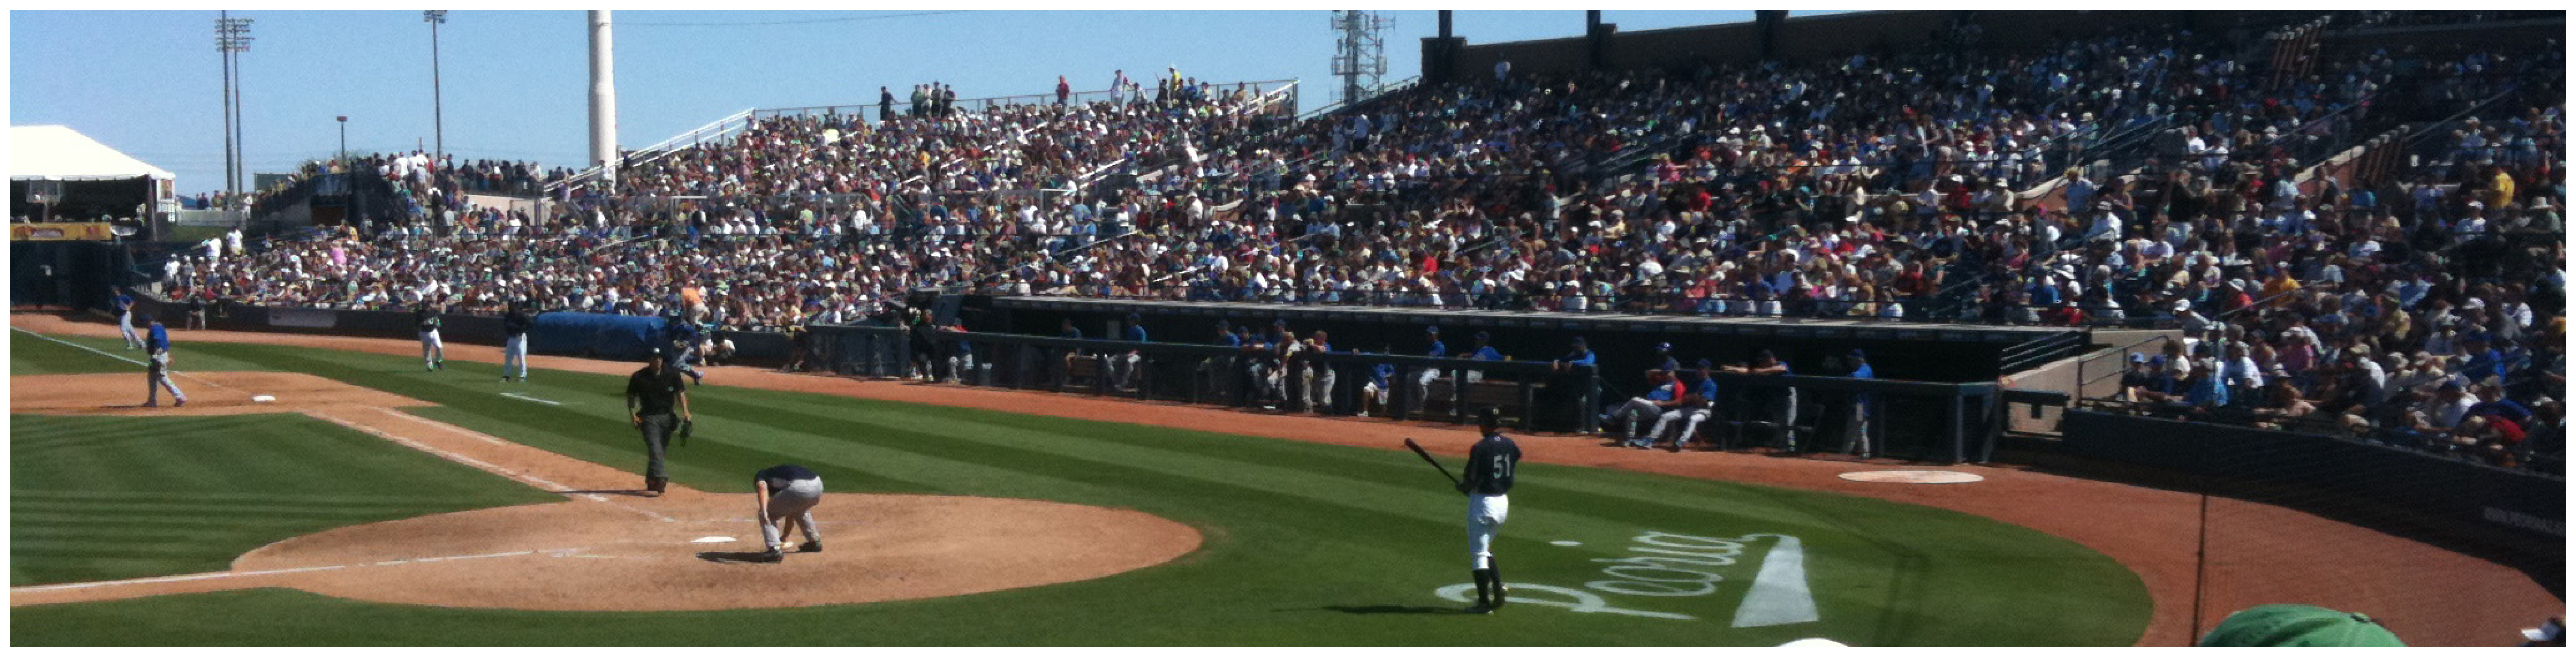
\includegraphics[height=1.5in]{images/sampleteaser}
%%   \caption{Spring Training 2009, Peoria, AZ.}
%% }

\maketitle

\begin{abstract}

.....

\end{abstract}

\copyrightspace

\section{Introduction}

\begin{itemize}
\item motivation
\item{
	general description of project
	\begin{itemize}
	\item what is it
	\item dark room side
	\item CAVE-side
	\end{itemize}
}
\item entire team
\item aspects: arts vs. technology
\item how we find the concept
\item purpose of this paper
\end{itemize}

\section{Implementation}

\subsection{General Application Architecture}
\textit{Graphic}
\begin{itemize}
\item brief description of components
\end{itemize}

\cref{SEC:CFE}
\cref{FIG:SAMPLE}

\subsection{Network}
\begin{itemize}
\item Liblo + OSC
\end{itemize}

\subsection{Visualisation}
\begin{itemize}
\item CAVE
\item OpenSG
\end{itemize}

\subsection{Interaction}

\begin{itemize}
\item introduction
\item used technologies
\item evolution over time
\item{
	detailed description
	\begin{itemize}
	\item UML, Code
	\item API
	\item implementation
	\end{itemize}
}
\end{itemize}

\section{Conclusion \& Further Extensions}
\label{SEC:CFE}

\begin{equation}
 \sum_{j=1}^{z} j = \frac{z(z+1)}{2}
\end{equation}

\begin{eqnarray}
x & \ll & y_{1} + \cdots + y_{n} \\
  & \leq & z
\end{eqnarray}

\begin{figure}[ht]
  \centering
  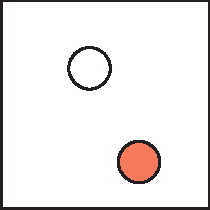
\includegraphics[width=1.5in]{images/samplefigure}
  \caption{Sample illustration.}
  \label{FIG:SAMPLE}
\end{figure}

\section*{Acknowledgements}

To my mum, my dad, and the dog. 

\bibliographystyle{acmsiggraph}
\bibliography{template}
\end{document}
